	\chapter{Introduction}
	Internet of Things (IoT) is a neologism, introduced by Kevin Ashton in 1999, which has become popular in recent years due to
	growing interest from companies the fact that nowadays it is possible to produce small devices with a reasonable computational power;
	these small devices are embedded in objects in order to make them, in some way, ``\emph{smart}''.\\
	
	IoT has a variety of different applications; ranging from everyday things like watches that measure how many kilometers we have walked during the day, to smart homes that control the air conditioning system based on temperature and pollution in the air, or even smart cities where semaphores adjust their times based on traffic condition.\\
	But these are only three examples, IoT extends also to other field like health care, industrial monitoring, self driving cars and agriculture.\\
	
	The IoT is also changing the way software is developed: in order to produce a good IoT system companies are required to cooperate each other,
	moving from a one-company-does-it-all perspective to a let’s-work-together approach ~\cite{successiot}, this means that proprietary systems 
	are no more a good choice and companies should embrace open systems in order to cooperate in a better way.\\
	
	From a financial point of view, IoT seems like a very profitable market, it is estimated that the global IoT market will grow to \$457B by 2020 ~\cite{forbes},by assuming this forecast as real, it means that lots of devices will be deployed in the network. Exposing a device
	or an host on the Internet also means exposing it to possible threats.\\
	An interesting case of insecure IoT system is given by a luxury hotel in Austria ~\cite{whydoiot}: the electronic key system was attacked
	by hacker that locked out (or in, it depends) guests from their rooms, until they paid a ransom.
	Long story short: after the attack, the hotel reverted to physical keys.\\
	Starting from this real case scenario we can imagine other problematic situations that does not imply an attack, for instance: if a blackout occurs, can a guest still access his well paid room?\\
	What if the content of the electronic key is not encrypted and it is possible to change its content in order to access other guests' room?\\
	This event should also make us think if we really need an IoT system for every aspects of our life: an electronic key system is
	surely comfortable, you can configure the electronic key as you want in few seconds, on the other hand it is quite easy to overwrite the content
	of an electronic key, while it is a bit more difficult to craft the copy of a physical key (if you are not a professional burglar), because you first need to steal it and duplicate it.\\
	Another interesting and funny case of insecure devices is provided by CloudPets\cite{toys} a company that produces toys, and in particular: Internet-connected fluffy animals toys.
	These toys were able to connect via Bluetooth to a smartphone's app in order to download and upload audio messages and it is possible to access the voice recordings without any authentication if you known the exact URL at which they were stored.\\
	The Guardian states that ``The personal information of more than half a million people who bought Internet-connected fluffy animals has been compromised'', it does not sounds like a good advertisement
	when the personal informations are: username, password, profile pictures and voice recordings.\\
	\textbf{Note:} the passwords were cracked easily because they were extremely easy to guess (``password'', ``123456'',``qwerty'', ``qwerty123456'' and so on).\\
	Another interesting thing to highlight is that "The personal information was contained in a database connected directly to the Internet, with no usernames or passwords preventing any visitor from accessing all the data", this could mean that the entire application was developed without any security requirements or security knowledge.\\
	 
	The security aspect of an IoT application is not only related to external attack by criminals but it also extends to reliability. Think about a power plant monitored by
	an IoT system: if it is not well designed and for some reason it does not take the proper countermeasures to avoid an overload, a blackout can occur and the consequences can be very bad, mostly from the financial point of view.\\
	These are the reasons why I am interested in analyzing the security aspect of IoT applications, considering that in near future
	IoT could be integral part of our lives I think it is crucial to develop secure systems.
	
	
	\section{Structure of an IoT application}
	Most of the time an IoT system is a large scale application that put in place different protocols, hardware and software.\newline
	From the protocol point of view there are lots of choices, just to list some of them: HTTP, MQTT, WebSocket and CoAP;
	each one has advantages and disadvantages, so it is crucial to choose the one that fits well your business logic; also taking in mind
	that some protocols, like MQTT or CoAP, are used in sensors-server communications, while HTTP and WebSocket
	are used for client-server communications.\newline
	While dealing with IoT we encounter a plethora of different hardware: from the constrained device with low computational power to
	high performance cluster machines. Basically the dirty work is taken over by lots of low power devices which communicate with the server,
	that will elaborate this data or forward it to the cloud in order to elaborate them in a faster way.\newline
	On the software front we can work with a variety of programming languages: from low level assembly to high level languages like C\# or JavaScript.\newline
	The development of an IoT system also requires a deep knowledge of different parts of an application, so the development team
	should consist of people with different skill and specialization.\newline
	This little overview should help you to understand how difficult could be to design and develop an IoT application; figure \ref{fig:intro0} illustrates a schema of the architecture of an IoT application.\newline
	
	\begin{figure}
		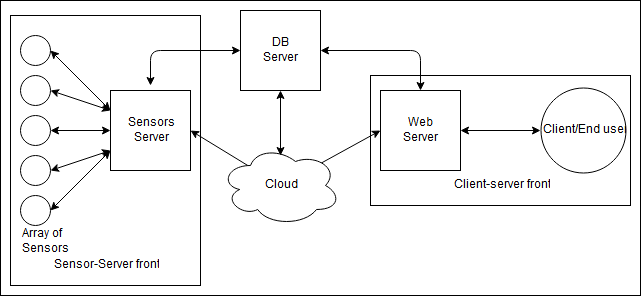
\includegraphics[width=\linewidth]{intro-000.png}
		\caption{Possible architecture of an IoT application.}
		\label{fig:intro0}
	\end{figure}
	
	\section{Covered topics}
	
	This thesis analyzes two IoT protocols: CoAP and WebSocket.\newline
	I chose these two protocols because they allow me to show how communication occurs on two different front:
	\begin{itemize}
		\item the sensor-server; where the server collects incoming data from the sensors, then the server proceed with some elaborations;
		\item and the client-server front, where the client requests data from the server in order to show them to the final user.
	\end{itemize}

	CoAP, described in chapter \ref{ch:coap}, is a protocol that works on the sensor-server part of the application, while WebSocket, described in chapter \ref{ch:ws}, focus
	on the client/server side. WebSocket is more flexible compared to CoAP, it can be used for
	jobs that where not taken into account during its design phase, while CoAP is a very specialized
	protocol that suits well only in certain constrained scenarios.\newline
	WebSocket can be used on the sensor-server side but, as we will analyze in details in the next chapter,
	we are going to deal with constrained devices that may lack the proper resources to implement the protocol.\newline
	
	After analyzing the two protocols, in chapter \ref{ch:vuln} we will focus on their vulnerabilities and possible attacks to show
	how important is to use them in a correct way in order to achieve security in IoT applications.\newline
	It is important to highlight that both communications: sensors-server and client-server must be secure in order to guarantee
	the security of the whole application, if the sensors-server is secure but the client-server is not, then an
	attacker could compromise the entire application while acting only on one front; of course this is true even for the other way around.\newline
	
	For the client-server front, in chapter \ref{ch:best},we will list the best practice to write a secure application, this section of the thesis
	is a mix of previous knowledges learned during the security course attended in the first year of the MsC and new one
	acquired during the internship at Abo Data.\newline
	
	In chapter \ref{ch:end} we will describe the experience in the company and draw some conclusion. We will discuss about two real IoT applications in order to have an in-depth overview of IoT applications.\newline
	Then we will describe the security flaws detected and how it was possible to fix them and evaluate how difficult it was.\newline
	We will analyze how security influences the development of an application and the reasons why sometimes it is neglected,
	in the end I will discuss how security should be an important part during the design and development phase of an application
	and not a final add-on for the system.\newline
	